\documentclass[main.tex]{subfiles}

\begin{document}

% \textcolor{red}{Вводная лекция}

\section{Лекция 16.02.2021 (Донцов Е.В.)}

План на сегодня: рассказать про основные компоненты моделирования ГРП (HF = hydraulic fracturing), про основные уравнения и основные геометрии.

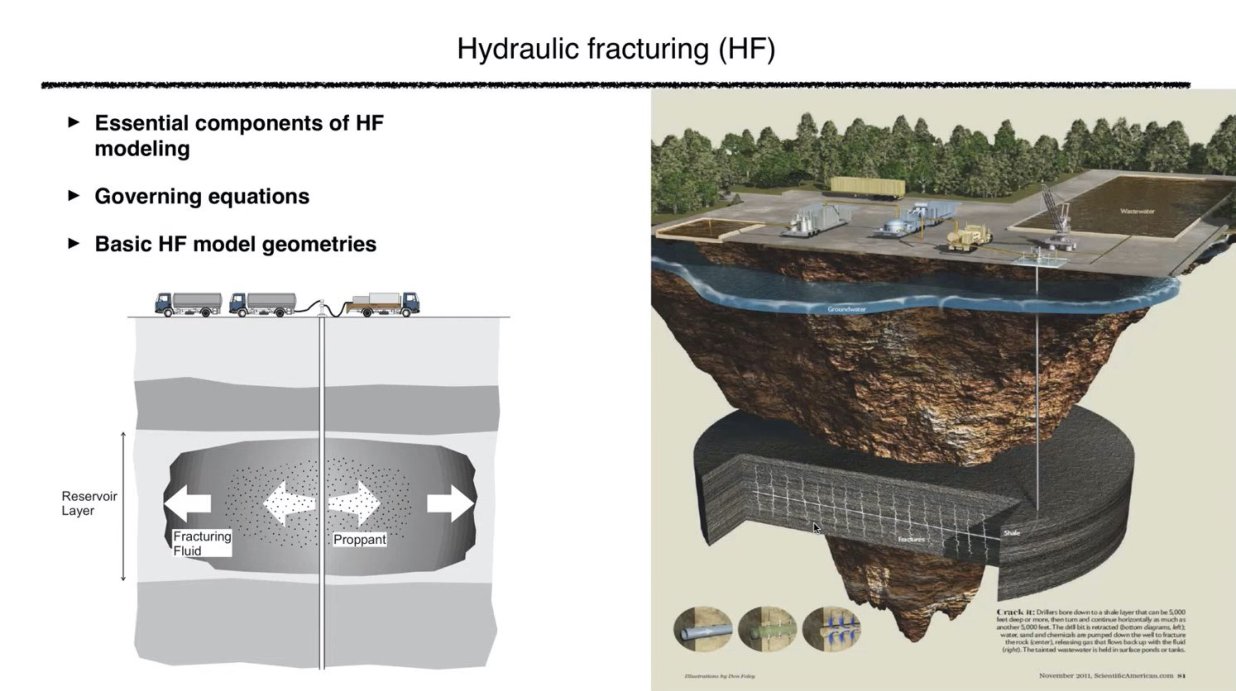
\includegraphics[width=\textwidth, page=1]{HF_slides.pdf}

В двух словах разница между conventional и unconventional:

1) conventional -- то, что было, грубо говоря, до 2000-х годов -- вертикальная скважина, пласт, рвём гидроразрывом пласта, обычно одна трещина

2) unconventional -- когда сланцы, например, то бурится горизонтальная скважина, проводится многостадийный ГРП (за одну стадию можем сделать несколько трещин, затем поставить перегородку, сделать ещё несколько трещин и так далее); можем также сделать несколько скважин

Концептуально с точки зрения математики разницы между conventional и unconventional практически нет.
У нас либо одна трещина (conventional) или множество трещин (unconventional), т.е. с точки зрения моделирования unconventional моделировать дольше, сложнее.
Но повторюсь, что концептуально основная физика везде одинакова.

\subsection{Из чего состоит любая модель ГРП? Основные компоненты}

\includegraphics[width=\textwidth, page=2]{HF_slides.pdf}

Основные компоненты любой модели гидроразрыва пласта:

1) закон сохранения жидкости; в 99\% случаев предполагается, что жидкость несжимаема, тогда выполняется закон сохранения объёма; но бывают случаи сжимаемых жидкостей (например, когда ГРП делают газом или делают пенный ГРП), тогда выполняется закон сохранения массы, т.е. закачиваемый объём жидкости равен объёму жидкости в трещине плюс утечки (трещину ГРП делаем в пористом резервуаре, поэтому есть утечки из трещины в резервуар -- в зависимости от пористости и других параметров утечки могут либо доминировать, либо нет);

2) уравнение течения жидкости в трещине; 

3) равновесие (упругость) горной породы;

4) условие распространения трещины;

5) транспорт проппанта

\subsection{Модель утечки по Картеру}

\includegraphics[width=\textwidth, page=3]{HF_slides.pdf}

\includegraphics[width=\textwidth, page=4]{HF_slides.pdf}

\includegraphics[width=\textwidth, page=5]{HF_slides.pdf}

\subsection{Течение жидкости}

\includegraphics[width=\textwidth, page=6]{HF_slides.pdf}

\subsection{Равновесие (упругость) горной породы}

\includegraphics[width=\textwidth, page=7]{HF_slides.pdf}



\end{document}